\documentclass[twoside]{book}

% Packages required by doxygen
\usepackage{calc}
\usepackage{doxygen}
\usepackage{graphicx}
\usepackage[utf8]{inputenc}
\usepackage{makeidx}
\usepackage{multicol}
\usepackage{multirow}
\usepackage{textcomp}
\usepackage[table]{xcolor}

% Font selection
\usepackage[T1]{fontenc}
\usepackage{mathptmx}
\usepackage[scaled=.90]{helvet}
\usepackage{courier}
\usepackage{amssymb}
\usepackage{sectsty}
\renewcommand{\familydefault}{\sfdefault}
\allsectionsfont{%
  \fontseries{bc}\selectfont%
  \color{darkgray}%
}
\renewcommand{\DoxyLabelFont}{%
  \fontseries{bc}\selectfont%
  \color{darkgray}%
}

% Page & text layout
\usepackage{geometry}
\geometry{%
  a4paper,%
  top=2.5cm,%
  bottom=2.5cm,%
  left=2.5cm,%
  right=2.5cm%
}
\tolerance=750
\hfuzz=15pt
\hbadness=750
\setlength{\emergencystretch}{15pt}
\setlength{\parindent}{0cm}
\setlength{\parskip}{0.2cm}
\makeatletter
\renewcommand{\paragraph}{%
  \@startsection{paragraph}{4}{0ex}{-1.0ex}{1.0ex}{%
    \normalfont\normalsize\bfseries\SS@parafont%
  }%
}
\renewcommand{\subparagraph}{%
  \@startsection{subparagraph}{5}{0ex}{-1.0ex}{1.0ex}{%
    \normalfont\normalsize\bfseries\SS@subparafont%
  }%
}
\makeatother

% Headers & footers
\usepackage{fancyhdr}
\pagestyle{fancyplain}
\fancyhead[LE]{\fancyplain{}{\bfseries\thepage}}
\fancyhead[CE]{\fancyplain{}{}}
\fancyhead[RE]{\fancyplain{}{\bfseries\leftmark}}
\fancyhead[LO]{\fancyplain{}{\bfseries\rightmark}}
\fancyhead[CO]{\fancyplain{}{}}
\fancyhead[RO]{\fancyplain{}{\bfseries\thepage}}
\fancyfoot[LE]{\fancyplain{}{}}
\fancyfoot[CE]{\fancyplain{}{}}
\fancyfoot[RE]{\fancyplain{}{\bfseries\scriptsize Generated on Tue May 19 2015 16\-:11\-:54 for Obserwator by Doxygen }}
\fancyfoot[LO]{\fancyplain{}{\bfseries\scriptsize Generated on Tue May 19 2015 16\-:11\-:54 for Obserwator by Doxygen }}
\fancyfoot[CO]{\fancyplain{}{}}
\fancyfoot[RO]{\fancyplain{}{}}
\renewcommand{\footrulewidth}{0.4pt}
\renewcommand{\chaptermark}[1]{%
  \markboth{#1}{}%
}
\renewcommand{\sectionmark}[1]{%
  \markright{\thesection\ #1}%
}

% Indices & bibliography
\usepackage{natbib}
\usepackage[titles]{tocloft}
\setcounter{tocdepth}{3}
\setcounter{secnumdepth}{5}
\makeindex

% Hyperlinks (required, but should be loaded last)
\usepackage{ifpdf}
\ifpdf
  \usepackage[pdftex,pagebackref=true]{hyperref}
\else
  \usepackage[ps2pdf,pagebackref=true]{hyperref}
\fi
\hypersetup{%
  colorlinks=true,%
  linkcolor=blue,%
  citecolor=blue,%
  unicode%
}

% Custom commands
\newcommand{\clearemptydoublepage}{%
  \newpage{\pagestyle{empty}\cleardoublepage}%
}


%===== C O N T E N T S =====

\begin{document}

% Titlepage & ToC
\hypersetup{pageanchor=false}
\pagenumbering{roman}
\begin{titlepage}
\vspace*{7cm}
\begin{center}%
{\Large Obserwator \\[1ex]\large 1 }\\
\vspace*{1cm}
{\large Generated by Doxygen 1.8.6}\\
\vspace*{0.5cm}
{\small Tue May 19 2015 16:11:54}\\
\end{center}
\end{titlepage}
\clearemptydoublepage
\tableofcontents
\clearemptydoublepage
\pagenumbering{arabic}
\hypersetup{pageanchor=true}

%--- Begin generated contents ---
\chapter{Hierarchical Index}
\section{Class Hierarchy}
This inheritance list is sorted roughly, but not completely, alphabetically\-:\begin{DoxyCompactList}
\item \contentsline{section}{Dane}{\pageref{class_dane}}{}
\begin{DoxyCompactList}
\item \contentsline{section}{Pobieracz\-Danych}{\pageref{class_pobieracz_danych}}{}
\end{DoxyCompactList}
\item \contentsline{section}{Ekolejka}{\pageref{struct_ekolejka}}{}
\item \contentsline{section}{Element}{\pageref{struct_element}}{}
\item \contentsline{section}{Graf}{\pageref{class_graf}}{}
\item \contentsline{section}{Kolejka}{\pageref{class_kolejka}}{}
\item \contentsline{section}{Ltab}{\pageref{class_ltab}}{}
\item \contentsline{section}{Obserwowany}{\pageref{class_obserwowany}}{}
\begin{DoxyCompactList}
\item \contentsline{section}{Obserwator}{\pageref{class_obserwator}}{}
\end{DoxyCompactList}
\item \contentsline{section}{Stos}{\pageref{class_stos}}{}
\end{DoxyCompactList}

\chapter{Class Index}
\section{Class List}
Here are the classes, structs, unions and interfaces with brief descriptions\-:\begin{DoxyCompactList}
\item\contentsline{section}{{\bf cegla} \\*Struktura pomocnicza cegla }{\pageref{structcegla}}{}
\item\contentsline{section}{{\bf ls\-::\-Kolejka} }{\pageref{classls_1_1_kolejka}}{}
\item\contentsline{section}{{\bf arr\-::\-Kolejka} }{\pageref{classarr_1_1_kolejka}}{}
\item\contentsline{section}{{\bf ls\-::\-Kontener} }{\pageref{classls_1_1_kontener}}{}
\item\contentsline{section}{{\bf arr\-::\-Lista} }{\pageref{classarr_1_1_lista}}{}
\item\contentsline{section}{{\bf ls\-::\-Stos} }{\pageref{classls_1_1_stos}}{}
\item\contentsline{section}{{\bf arr\-::\-Stos} }{\pageref{classarr_1_1_stos}}{}
\end{DoxyCompactList}

\chapter{File Index}
\section{File List}
Here is a list of all files with brief descriptions\-:\begin{DoxyCompactList}
\item\contentsline{section}{/home/damian/prog/praca na zajeciach(nowy sort)/\-Sortowania(wybrany-\/przez wstawianie)/prj/inc/\hyperlink{_lista_ar_8h}{Lista\-Ar.\-h} \\*Plik naglowkowy \hyperlink{_lista_ar_8h}{Lista\-Ar.\-h} }{\pageref{_lista_ar_8h}}{}
\item\contentsline{section}{/home/damian/prog/praca na zajeciach(nowy sort)/\-Sortowania(wybrany-\/przez wstawianie)/prj/src/\hyperlink{_lista_ar_8cpp}{Lista\-Ar.\-cpp} \\*Plik \hyperlink{_lista_ar_8cpp}{Lista\-Ar.\-cpp} }{\pageref{_lista_ar_8cpp}}{}
\item\contentsline{section}{/home/damian/prog/praca na zajeciach(nowy sort)/\-Sortowania(wybrany-\/przez wstawianie)/prj/src/\hyperlink{main_8cpp}{main.\-cpp} \\*Plik \hyperlink{main_8cpp}{main.\-cpp} }{\pageref{main_8cpp}}{}
\end{DoxyCompactList}

\chapter{Class Documentation}
\hypertarget{class_dane}{\section{Dane Class Reference}
\label{class_dane}\index{Dane@{Dane}}
}


Deklaracja klasy \hyperlink{class_dane}{Dane}.  




{\ttfamily \#include $<$Benchmark.\-h$>$}

Inheritance diagram for Dane\-:\begin{figure}[H]
\begin{center}
\leavevmode
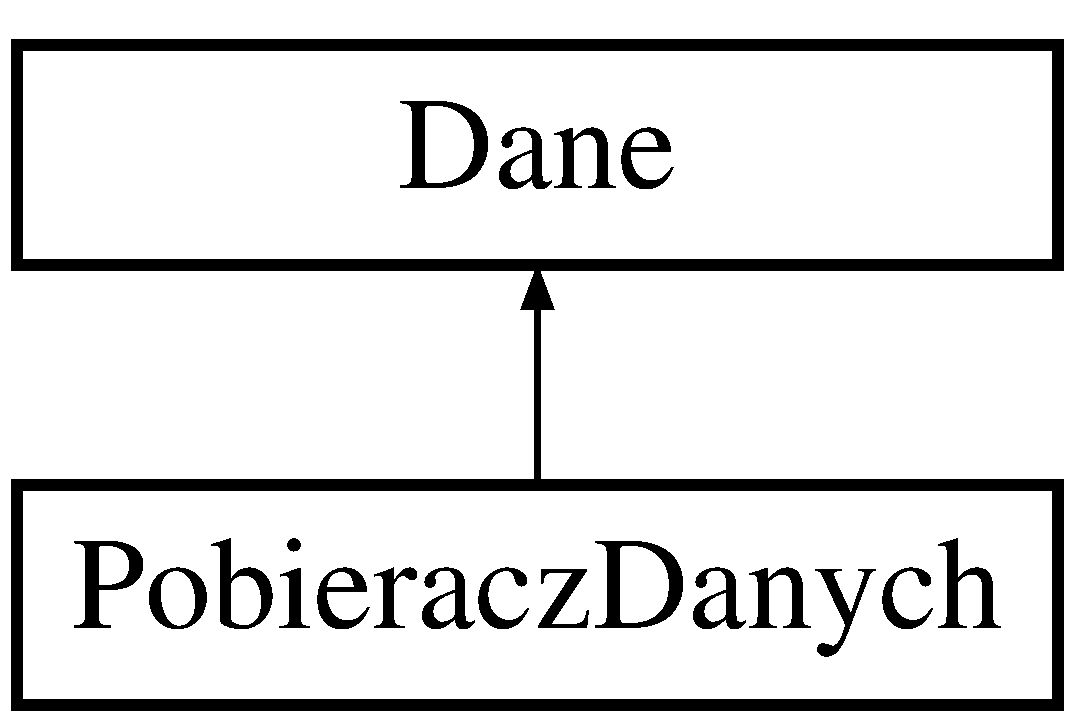
\includegraphics[height=2.000000cm]{class_dane}
\end{center}
\end{figure}
\subsection*{Public Member Functions}
\begin{DoxyCompactItemize}
\item 
virtual void \hyperlink{class_dane_a45055e5aa4e72fbb3a0717447fafbe75}{update} (\hyperlink{class_obserwowany}{Obserwowany} $\ast$)=0
\end{DoxyCompactItemize}


\subsection{Detailed Description}
Deklaracja klasy \hyperlink{class_dane}{Dane}. 

Jest to obserwator 

Definition at line 34 of file Benchmark.\-h.



\subsection{Member Function Documentation}
\hypertarget{class_dane_a45055e5aa4e72fbb3a0717447fafbe75}{\index{Dane@{Dane}!update@{update}}
\index{update@{update}!Dane@{Dane}}
\subsubsection[{update}]{\setlength{\rightskip}{0pt plus 5cm}virtual void Dane\-::update (
\begin{DoxyParamCaption}
\item[{{\bf Obserwowany} $\ast$}]{}
\end{DoxyParamCaption}
)\hspace{0.3cm}{\ttfamily [pure virtual]}}}\label{class_dane_a45055e5aa4e72fbb3a0717447fafbe75}


Implemented in \hyperlink{class_pobieracz_danych_a36a1901f8c7f9228f90c713a8e267b98}{Pobieracz\-Danych}.



The documentation for this class was generated from the following file\-:\begin{DoxyCompactItemize}
\item 
/home/damian/prog/\-Obserwator/prj/inc/\hyperlink{_benchmark_8h}{Benchmark.\-h}\end{DoxyCompactItemize}

\hypertarget{class_ltab}{\section{Ltab Class Reference}
\label{class_ltab}\index{Ltab@{Ltab}}
}


Modeluje pojecie klasy \hyperlink{class_ltab}{Ltab}.  




{\ttfamily \#include $<$Lista\-Ar.\-h$>$}

\subsection*{Public Member Functions}
\begin{DoxyCompactItemize}
\item 
\hyperlink{class_ltab_ab6cfd85d06ae19d676c3057dcd119541}{Ltab} ()
\begin{DoxyCompactList}\small\item\em Konstruktor klasy \hyperlink{class_ltab}{Ltab}. \end{DoxyCompactList}\item 
\hyperlink{class_ltab_a964bb07c6108ab0bcd31e4ae7d8ea35a}{Ltab} (const \hyperlink{class_ltab}{Ltab} \&w)
\begin{DoxyCompactList}\small\item\em Konstruktor kopjujacy klasy \hyperlink{class_ltab}{Ltab}. \end{DoxyCompactList}\item 
\hyperlink{class_ltab_af01a96400af8f3988c8a2800ce0eae22}{$\sim$\-Ltab} ()
\begin{DoxyCompactList}\small\item\em Destruktor klasy \hyperlink{class_ltab}{Ltab}. \end{DoxyCompactList}\item 
\hyperlink{class_ltab}{Ltab} \& \hyperlink{class_ltab_a174a5a31161a157d7724e560b99ad170}{operator=} (const \hyperlink{class_ltab}{Ltab} \&w)
\begin{DoxyCompactList}\small\item\em Przeciazenie operatora = dla klasy \hyperlink{class_ltab}{Ltab}. \end{DoxyCompactList}\item 
int \& \hyperlink{class_ltab_a3e6dae99d55dcaf9ead923a5588c3d57}{operator\mbox{[}$\,$\mbox{]}} (unsigned int index)
\begin{DoxyCompactList}\small\item\em Przeciazenie operatora \mbox{[}\mbox{]} dla klasy \hyperlink{class_ltab}{Ltab}. \end{DoxyCompactList}\item 
void \hyperlink{class_ltab_a9d984316c3c88691e9ccfeaed884bfff}{add} (const int \&wart)
\begin{DoxyCompactList}\small\item\em Metoda klasy \hyperlink{class_ltab}{Ltab} add. \end{DoxyCompactList}\item 
void \hyperlink{class_ltab_ade764d08f90e2989bef67a652202f9f1}{addx2} (const int \&wart)
\begin{DoxyCompactList}\small\item\em Metoda klasy \hyperlink{class_ltab}{Ltab} addx2. \end{DoxyCompactList}\item 
void \hyperlink{class_ltab_a4b81c405bc3cf4b4510b0e879ec983b2}{wypisz} ()
\begin{DoxyCompactList}\small\item\em Metoda klasy \hyperlink{class_ltab}{Ltab} wypisz. \end{DoxyCompactList}\item 
void \hyperlink{class_ltab_adc068a9b92a287cdd0b57497b9859eca}{sort\-\_\-wst} ()
\begin{DoxyCompactList}\small\item\em Metoda klasy \hyperlink{class_ltab}{Ltab} sort\-\_\-wst. \end{DoxyCompactList}\item 
int \hyperlink{class_ltab_a83fcc265ec39c5a78826118e86aaddc2}{dziel} (int lewo, int prawo)
\begin{DoxyCompactList}\small\item\em Metoda klasy \hyperlink{class_ltab}{Ltab} dziel. \end{DoxyCompactList}\item 
int \hyperlink{class_ltab_aadee500f6112321d8664f3989daf37df}{dziel2} (int lewo, int prawo)
\begin{DoxyCompactList}\small\item\em Metoda klasy \hyperlink{class_ltab}{Ltab} dziel2. \end{DoxyCompactList}\item 
void \hyperlink{class_ltab_a3fbc0651b0d2c4592357e4028ff5a0f7}{sortuj} (int lewo, int prawo)
\begin{DoxyCompactList}\small\item\em Metoda klasy \hyperlink{class_ltab}{Ltab} sortuj. \end{DoxyCompactList}\item 
void \hyperlink{class_ltab_a30e46ca8cc5bada27cf3f7d2eedce4d1}{sortuj\-\_\-opt} (int lewo, int prawo)
\begin{DoxyCompactList}\small\item\em Metoda klasy \hyperlink{class_ltab}{Ltab} sortuj\-\_\-opt. \end{DoxyCompactList}\item 
void \hyperlink{class_ltab_a57d2fa20504b7dda2f6be20e26679aef}{sort\-\_\-scal} (int lewo, int prawo)
\begin{DoxyCompactList}\small\item\em Metoda klasy \hyperlink{class_ltab}{Ltab} sort\-\_\-scal. \end{DoxyCompactList}\item 
void \hyperlink{class_ltab_a16b62be673fff8092ec63b83c0e3bdca}{scal} (int lewo, int srodek, int prawo)
\begin{DoxyCompactList}\small\item\em Metoda klasy \hyperlink{class_ltab}{Ltab} scal. \end{DoxyCompactList}\item 
void \hyperlink{class_ltab_a414506ad786eddec135a51cce17e1edb}{sort\-\_\-hybr} (int lewo, int prawo)
\begin{DoxyCompactList}\small\item\em Metoda klasy \hyperlink{class_ltab}{Ltab} sort\-\_\-hybr. \end{DoxyCompactList}\item 
void \hyperlink{class_ltab_a503a8f38c9533941551261d3d5403ea4}{wypelnij\-\_\-posortowane} (int roz)
\begin{DoxyCompactList}\small\item\em Metoda klasy \hyperlink{class_ltab}{Ltab} wypelnij\-\_\-posortowane. \end{DoxyCompactList}\item 
void \hyperlink{class_ltab_a198bbbe58da442f53b233e2e8a7e170a}{wypelnij\-\_\-odwrotnie} (int roz)
\begin{DoxyCompactList}\small\item\em Metoda klasy \hyperlink{class_ltab}{Ltab} wypelnij\-\_\-odwrotnie. \end{DoxyCompactList}\item 
void \hyperlink{class_ltab_a7fb9b7832172a4e6ec1f4b2e2a582c63}{wypelnij\-\_\-losowymi} (int roz)
\begin{DoxyCompactList}\small\item\em Metoda klasy \hyperlink{class_ltab}{Ltab} wypelnij\-\_\-losowymi. \end{DoxyCompactList}\item 
void \hyperlink{class_ltab_acc8c695848136fdfef9099951c3a2c45}{sortuj\-\_\-\-Q\-S\-\_\-wst} (int lewo, int prawo)
\begin{DoxyCompactList}\small\item\em Metoda klasy \hyperlink{class_ltab}{Ltab} sortuj\-\_\-\-Q\-S\-\_\-wst. \end{DoxyCompactList}\end{DoxyCompactItemize}


\subsection{Detailed Description}
Modeluje pojecie klasy \hyperlink{class_ltab}{Ltab}. 

Klasa \hyperlink{class_ltab}{Ltab} zawiera prywatnie ilosc elementow w tablicy, maksynalna ilosc elementow w tablicy oraz element Publicznie zawieraz wszystkie metody, przeciazenia operatorow oraz konstruktor i destruktor. 

Definition at line 22 of file Lista\-Ar.\-h.



\subsection{Constructor \& Destructor Documentation}
\hypertarget{class_ltab_ab6cfd85d06ae19d676c3057dcd119541}{\index{Ltab@{Ltab}!Ltab@{Ltab}}
\index{Ltab@{Ltab}!Ltab@{Ltab}}
\subsubsection[{Ltab}]{\setlength{\rightskip}{0pt plus 5cm}Ltab\-::\-Ltab (
\begin{DoxyParamCaption}
{}
\end{DoxyParamCaption}
)}}\label{class_ltab_ab6cfd85d06ae19d676c3057dcd119541}


Konstruktor klasy \hyperlink{class_ltab}{Ltab}. 

Tworzy pusta klase \hyperlink{class_ltab}{Ltab} 

Definition at line 14 of file Lista\-Ar.\-cpp.

\hypertarget{class_ltab_a964bb07c6108ab0bcd31e4ae7d8ea35a}{\index{Ltab@{Ltab}!Ltab@{Ltab}}
\index{Ltab@{Ltab}!Ltab@{Ltab}}
\subsubsection[{Ltab}]{\setlength{\rightskip}{0pt plus 5cm}Ltab\-::\-Ltab (
\begin{DoxyParamCaption}
\item[{const {\bf Ltab} \&}]{w}
\end{DoxyParamCaption}
)}}\label{class_ltab_a964bb07c6108ab0bcd31e4ae7d8ea35a}


Konstruktor kopjujacy klasy \hyperlink{class_ltab}{Ltab}. 

Kopjuje cala list

\begin{DoxyReturn}{Returns}
Zwraca klase \hyperlink{class_ltab}{Ltab} 
\end{DoxyReturn}


Definition at line 74 of file Lista\-Ar.\-cpp.

\hypertarget{class_ltab_af01a96400af8f3988c8a2800ce0eae22}{\index{Ltab@{Ltab}!$\sim$\-Ltab@{$\sim$\-Ltab}}
\index{$\sim$\-Ltab@{$\sim$\-Ltab}!Ltab@{Ltab}}
\subsubsection[{$\sim$\-Ltab}]{\setlength{\rightskip}{0pt plus 5cm}Ltab\-::$\sim$\-Ltab (
\begin{DoxyParamCaption}
{}
\end{DoxyParamCaption}
)}}\label{class_ltab_af01a96400af8f3988c8a2800ce0eae22}


Destruktor klasy \hyperlink{class_ltab}{Ltab}. 

Kasuje cala klase 

Definition at line 22 of file Lista\-Ar.\-cpp.



\subsection{Member Function Documentation}
\hypertarget{class_ltab_a9d984316c3c88691e9ccfeaed884bfff}{\index{Ltab@{Ltab}!add@{add}}
\index{add@{add}!Ltab@{Ltab}}
\subsubsection[{add}]{\setlength{\rightskip}{0pt plus 5cm}void Ltab\-::add (
\begin{DoxyParamCaption}
\item[{const int \&}]{wart}
\end{DoxyParamCaption}
)}}\label{class_ltab_a9d984316c3c88691e9ccfeaed884bfff}


Metoda klasy \hyperlink{class_ltab}{Ltab} add. 

Dodaje element do listy zwiekszajac jej rozmiar o 1


\begin{DoxyParams}[1]{Parameters}
\mbox{\tt in}  & {\em wart} & -\/ taka bedzie wartosc dodanego elementu \\
\hline
\end{DoxyParams}


Definition at line 29 of file Lista\-Ar.\-cpp.

\hypertarget{class_ltab_ade764d08f90e2989bef67a652202f9f1}{\index{Ltab@{Ltab}!addx2@{addx2}}
\index{addx2@{addx2}!Ltab@{Ltab}}
\subsubsection[{addx2}]{\setlength{\rightskip}{0pt plus 5cm}void Ltab\-::addx2 (
\begin{DoxyParamCaption}
\item[{const int \&}]{wart}
\end{DoxyParamCaption}
)}}\label{class_ltab_ade764d08f90e2989bef67a652202f9f1}


Metoda klasy \hyperlink{class_ltab}{Ltab} addx2. 

Dodaje element na szczyt listy jesli jest jeszcze miejsce w tablicy. Jesli nie to zwieksza rozmiar tablicy razy 2 a potem dodaje element


\begin{DoxyParams}[1]{Parameters}
\mbox{\tt in}  & {\em wart} & -\/ taka bedzie wartosc dodanego elementu \\
\hline
\end{DoxyParams}


Definition at line 50 of file Lista\-Ar.\-cpp.

\hypertarget{class_ltab_a83fcc265ec39c5a78826118e86aaddc2}{\index{Ltab@{Ltab}!dziel@{dziel}}
\index{dziel@{dziel}!Ltab@{Ltab}}
\subsubsection[{dziel}]{\setlength{\rightskip}{0pt plus 5cm}int Ltab\-::dziel (
\begin{DoxyParamCaption}
\item[{int}]{lewo, }
\item[{int}]{prawo}
\end{DoxyParamCaption}
)}}\label{class_ltab_a83fcc265ec39c5a78826118e86aaddc2}


Metoda klasy \hyperlink{class_ltab}{Ltab} dziel. 

Dzieli tablice na 2 czesci. Metoda wykorzystywana w metodzie sotrtuj \begin{DoxyReturn}{Returns}
Zwraca punkt podzialu tablicy Q\-S przerobiony z tego robionego pod program kolegi na dzialajacy na moim 
\end{DoxyReturn}


Definition at line 108 of file Lista\-Ar.\-cpp.

\hypertarget{class_ltab_aadee500f6112321d8664f3989daf37df}{\index{Ltab@{Ltab}!dziel2@{dziel2}}
\index{dziel2@{dziel2}!Ltab@{Ltab}}
\subsubsection[{dziel2}]{\setlength{\rightskip}{0pt plus 5cm}int Ltab\-::dziel2 (
\begin{DoxyParamCaption}
\item[{int}]{lewo, }
\item[{int}]{prawo}
\end{DoxyParamCaption}
)}}\label{class_ltab_aadee500f6112321d8664f3989daf37df}


Metoda klasy \hyperlink{class_ltab}{Ltab} dziel2. 

Dzieli tablice na 2 czesci. Metoda wykorzystywana w metodzie sotrtuj\-\_\-opt \begin{DoxyReturn}{Returns}
Zwraca punkt podzialu tablicy Q\-S przerobiony z tego robionego pod program kolegi na dzialajacy na moim 
\end{DoxyReturn}


Definition at line 145 of file Lista\-Ar.\-cpp.

\hypertarget{class_ltab_a174a5a31161a157d7724e560b99ad170}{\index{Ltab@{Ltab}!operator=@{operator=}}
\index{operator=@{operator=}!Ltab@{Ltab}}
\subsubsection[{operator=}]{\setlength{\rightskip}{0pt plus 5cm}{\bf Ltab} \& Ltab\-::operator= (
\begin{DoxyParamCaption}
\item[{const {\bf Ltab} \&}]{w}
\end{DoxyParamCaption}
)}}\label{class_ltab_a174a5a31161a157d7724e560b99ad170}


Przeciazenie operatora = dla klasy \hyperlink{class_ltab}{Ltab}. 

Przypisuje wartosci jednej listy do drugiej 

Definition at line 91 of file Lista\-Ar.\-cpp.

\hypertarget{class_ltab_a3e6dae99d55dcaf9ead923a5588c3d57}{\index{Ltab@{Ltab}!operator\mbox{[}$\,$\mbox{]}@{operator[]}}
\index{operator\mbox{[}$\,$\mbox{]}@{operator[]}!Ltab@{Ltab}}
\subsubsection[{operator[]}]{\setlength{\rightskip}{0pt plus 5cm}int \& Ltab\-::operator\mbox{[}$\,$\mbox{]} (
\begin{DoxyParamCaption}
\item[{unsigned int}]{index}
\end{DoxyParamCaption}
)}}\label{class_ltab_a3e6dae99d55dcaf9ead923a5588c3d57}


Przeciazenie operatora \mbox{[}\mbox{]} dla klasy \hyperlink{class_ltab}{Ltab}. 

Pozwala na odwolanie sie do elementu tablicy 

Definition at line 102 of file Lista\-Ar.\-cpp.

\hypertarget{class_ltab_a16b62be673fff8092ec63b83c0e3bdca}{\index{Ltab@{Ltab}!scal@{scal}}
\index{scal@{scal}!Ltab@{Ltab}}
\subsubsection[{scal}]{\setlength{\rightskip}{0pt plus 5cm}void Ltab\-::scal (
\begin{DoxyParamCaption}
\item[{int}]{lewo, }
\item[{int}]{srodek, }
\item[{int}]{prawo}
\end{DoxyParamCaption}
)}}\label{class_ltab_a16b62be673fff8092ec63b83c0e3bdca}


Metoda klasy \hyperlink{class_ltab}{Ltab} scal. 

Metoda sortuje elementy tablicy od najmniejsego do najwiekszego. Wykorzystuje algorytm scalania(merge) 

Definition at line 284 of file Lista\-Ar.\-cpp.

\hypertarget{class_ltab_a414506ad786eddec135a51cce17e1edb}{\index{Ltab@{Ltab}!sort\-\_\-hybr@{sort\-\_\-hybr}}
\index{sort\-\_\-hybr@{sort\-\_\-hybr}!Ltab@{Ltab}}
\subsubsection[{sort\-\_\-hybr}]{\setlength{\rightskip}{0pt plus 5cm}void Ltab\-::sort\-\_\-hybr (
\begin{DoxyParamCaption}
\item[{int}]{lewo, }
\item[{int}]{prawo}
\end{DoxyParamCaption}
)}}\label{class_ltab_a414506ad786eddec135a51cce17e1edb}


Metoda klasy \hyperlink{class_ltab}{Ltab} sort\-\_\-hybr. 

Metoda sortuje elementy tablicy od najmniejsego do najwiekszego.

Metoda ta wykorzystuje metode dziel oraz metode sort\-\_\-wst 

Definition at line 339 of file Lista\-Ar.\-cpp.

\hypertarget{class_ltab_a57d2fa20504b7dda2f6be20e26679aef}{\index{Ltab@{Ltab}!sort\-\_\-scal@{sort\-\_\-scal}}
\index{sort\-\_\-scal@{sort\-\_\-scal}!Ltab@{Ltab}}
\subsubsection[{sort\-\_\-scal}]{\setlength{\rightskip}{0pt plus 5cm}void Ltab\-::sort\-\_\-scal (
\begin{DoxyParamCaption}
\item[{int}]{lewo, }
\item[{int}]{prawo}
\end{DoxyParamCaption}
)}}\label{class_ltab_a57d2fa20504b7dda2f6be20e26679aef}


Metoda klasy \hyperlink{class_ltab}{Ltab} sort\-\_\-scal. 

Metoda scala dwie czesci tablicy w jedna 

Definition at line 315 of file Lista\-Ar.\-cpp.

\hypertarget{class_ltab_adc068a9b92a287cdd0b57497b9859eca}{\index{Ltab@{Ltab}!sort\-\_\-wst@{sort\-\_\-wst}}
\index{sort\-\_\-wst@{sort\-\_\-wst}!Ltab@{Ltab}}
\subsubsection[{sort\-\_\-wst}]{\setlength{\rightskip}{0pt plus 5cm}void Ltab\-::sort\-\_\-wst (
\begin{DoxyParamCaption}
{}
\end{DoxyParamCaption}
)}}\label{class_ltab_adc068a9b92a287cdd0b57497b9859eca}


Metoda klasy \hyperlink{class_ltab}{Ltab} sort\-\_\-wst. 

Sortuje elementy listy od najmniejszego do największego Zlozonosc algorytmu to O(n$^\wedge$2) dla samego algorytmu sortowania, gdzie n to ilosc elementow do posortowania, ale występuje tam rownierz kopjowanie calej zawartosci tablicy.

T\-A\-B\-E\-L\-A C\-Z\-A\-S\-O\-W

n czas\mbox{[}s\mbox{]} 100 0,000039 1000 0,003291 10000 0,016735 100000 15,6825 

Definition at line 252 of file Lista\-Ar.\-cpp.

\hypertarget{class_ltab_a3fbc0651b0d2c4592357e4028ff5a0f7}{\index{Ltab@{Ltab}!sortuj@{sortuj}}
\index{sortuj@{sortuj}!Ltab@{Ltab}}
\subsubsection[{sortuj}]{\setlength{\rightskip}{0pt plus 5cm}void Ltab\-::sortuj (
\begin{DoxyParamCaption}
\item[{int}]{lewo, }
\item[{int}]{prawo}
\end{DoxyParamCaption}
)}}\label{class_ltab_a3fbc0651b0d2c4592357e4028ff5a0f7}


Metoda klasy \hyperlink{class_ltab}{Ltab} sortuj. 

Metoda sortuje elementy tablicy od najmniejsego do najwiekszego. Jest to algorytm Q\-S

Q\-S przerobiony z tego robionego pod program kolegi na dzialajacy na moim 

Definition at line 228 of file Lista\-Ar.\-cpp.

\hypertarget{class_ltab_a30e46ca8cc5bada27cf3f7d2eedce4d1}{\index{Ltab@{Ltab}!sortuj\-\_\-opt@{sortuj\-\_\-opt}}
\index{sortuj\-\_\-opt@{sortuj\-\_\-opt}!Ltab@{Ltab}}
\subsubsection[{sortuj\-\_\-opt}]{\setlength{\rightskip}{0pt plus 5cm}void Ltab\-::sortuj\-\_\-opt (
\begin{DoxyParamCaption}
\item[{int}]{lewo, }
\item[{int}]{prawo}
\end{DoxyParamCaption}
)}}\label{class_ltab_a30e46ca8cc5bada27cf3f7d2eedce4d1}


Metoda klasy \hyperlink{class_ltab}{Ltab} sortuj\-\_\-opt. 

Metoda sortuje elementy tablicy od najmniejsego do najwiekszego. Jest to algorytm Q\-S z optymalizacja. Optymalizacja polega na doborze pivota. Jest on wybierany jako mediana 3 elementow -\/ pierwszego, srodkowego i ostatniego.

Q\-S przerobiony z tego robionego pod program kolegi na dzialajacy na moim 

Definition at line 239 of file Lista\-Ar.\-cpp.

\hypertarget{class_ltab_acc8c695848136fdfef9099951c3a2c45}{\index{Ltab@{Ltab}!sortuj\-\_\-\-Q\-S\-\_\-wst@{sortuj\-\_\-\-Q\-S\-\_\-wst}}
\index{sortuj\-\_\-\-Q\-S\-\_\-wst@{sortuj\-\_\-\-Q\-S\-\_\-wst}!Ltab@{Ltab}}
\subsubsection[{sortuj\-\_\-\-Q\-S\-\_\-wst}]{\setlength{\rightskip}{0pt plus 5cm}void Ltab\-::sortuj\-\_\-\-Q\-S\-\_\-wst (
\begin{DoxyParamCaption}
\item[{int}]{lewo, }
\item[{int}]{prawo}
\end{DoxyParamCaption}
)}}\label{class_ltab_acc8c695848136fdfef9099951c3a2c45}


Metoda klasy \hyperlink{class_ltab}{Ltab} sortuj\-\_\-\-Q\-S\-\_\-wst. 

Metoda wypelnia sortuje elementy tablicy od najmniejszego do najwiekszego. Wykorzystuje do tego w pierwszej kolejnosci metode dziel ktora dzieli elementy tablicy na dwie czesci i wstepnie je sortuje. Nastepnie dla wstepnie posortowanych elementow wywolywana jest metoda sort\-\_\-wst ktora ma zlozonosc linniowa dla elementow czesciowo posortowanych. 

Definition at line 329 of file Lista\-Ar.\-cpp.

\hypertarget{class_ltab_a7fb9b7832172a4e6ec1f4b2e2a582c63}{\index{Ltab@{Ltab}!wypelnij\-\_\-losowymi@{wypelnij\-\_\-losowymi}}
\index{wypelnij\-\_\-losowymi@{wypelnij\-\_\-losowymi}!Ltab@{Ltab}}
\subsubsection[{wypelnij\-\_\-losowymi}]{\setlength{\rightskip}{0pt plus 5cm}void Ltab\-::wypelnij\-\_\-losowymi (
\begin{DoxyParamCaption}
\item[{int}]{roz}
\end{DoxyParamCaption}
)}}\label{class_ltab_a7fb9b7832172a4e6ec1f4b2e2a582c63}


Metoda klasy \hyperlink{class_ltab}{Ltab} wypelnij\-\_\-losowymi. 

Metoda wypelnia tablice losowymi elementami z zakresu od 0 do 999 

Definition at line 349 of file Lista\-Ar.\-cpp.

\hypertarget{class_ltab_a198bbbe58da442f53b233e2e8a7e170a}{\index{Ltab@{Ltab}!wypelnij\-\_\-odwrotnie@{wypelnij\-\_\-odwrotnie}}
\index{wypelnij\-\_\-odwrotnie@{wypelnij\-\_\-odwrotnie}!Ltab@{Ltab}}
\subsubsection[{wypelnij\-\_\-odwrotnie}]{\setlength{\rightskip}{0pt plus 5cm}void Ltab\-::wypelnij\-\_\-odwrotnie (
\begin{DoxyParamCaption}
\item[{int}]{roz}
\end{DoxyParamCaption}
)}}\label{class_ltab_a198bbbe58da442f53b233e2e8a7e170a}


Metoda klasy \hyperlink{class_ltab}{Ltab} wypelnij\-\_\-odwrotnie. 

Metoda wypelnia tablice elementami od roz do 1 

Definition at line 360 of file Lista\-Ar.\-cpp.

\hypertarget{class_ltab_a503a8f38c9533941551261d3d5403ea4}{\index{Ltab@{Ltab}!wypelnij\-\_\-posortowane@{wypelnij\-\_\-posortowane}}
\index{wypelnij\-\_\-posortowane@{wypelnij\-\_\-posortowane}!Ltab@{Ltab}}
\subsubsection[{wypelnij\-\_\-posortowane}]{\setlength{\rightskip}{0pt plus 5cm}void Ltab\-::wypelnij\-\_\-posortowane (
\begin{DoxyParamCaption}
\item[{int}]{roz}
\end{DoxyParamCaption}
)}}\label{class_ltab_a503a8f38c9533941551261d3d5403ea4}


Metoda klasy \hyperlink{class_ltab}{Ltab} wypelnij\-\_\-posortowane. 

Metoda wypelnia tablice elementami od 1 do roz 

Definition at line 372 of file Lista\-Ar.\-cpp.

\hypertarget{class_ltab_a4b81c405bc3cf4b4510b0e879ec983b2}{\index{Ltab@{Ltab}!wypisz@{wypisz}}
\index{wypisz@{wypisz}!Ltab@{Ltab}}
\subsubsection[{wypisz}]{\setlength{\rightskip}{0pt plus 5cm}void Ltab\-::wypisz (
\begin{DoxyParamCaption}
{}
\end{DoxyParamCaption}
)}}\label{class_ltab_a4b81c405bc3cf4b4510b0e879ec983b2}


Metoda klasy \hyperlink{class_ltab}{Ltab} wypisz. 

Wyswietla cala zawartosc listy 

Definition at line 84 of file Lista\-Ar.\-cpp.



The documentation for this class was generated from the following files\-:\begin{DoxyCompactItemize}
\item 
/home/damian/prog/\-Obserwator/prj/inc/\hyperlink{_lista_ar_8h}{Lista\-Ar.\-h}\item 
/home/damian/prog/\-Obserwator/prj/src/\hyperlink{_lista_ar_8cpp}{Lista\-Ar.\-cpp}\end{DoxyCompactItemize}

\hypertarget{class_obserwator}{\section{Obserwator Class Reference}
\label{class_obserwator}\index{Obserwator@{Obserwator}}
}


Definicja klasy \hyperlink{class_obserwator}{Obserwator}.  




{\ttfamily \#include $<$Benchmark.\-h$>$}

Inheritance diagram for Obserwator\-:\begin{figure}[H]
\begin{center}
\leavevmode
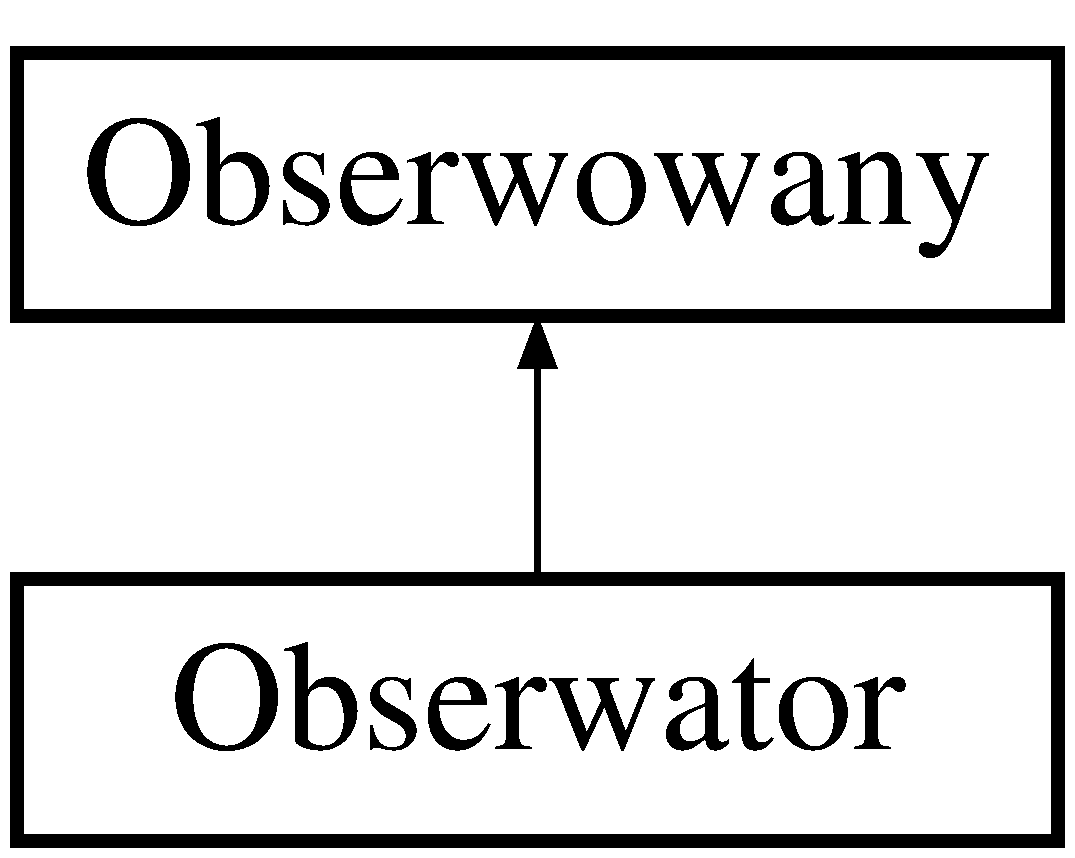
\includegraphics[height=2.000000cm]{class_obserwator}
\end{center}
\end{figure}
\subsection*{Public Member Functions}
\begin{DoxyCompactItemize}
\item 
\hyperlink{class_obserwator_a48222b9c0db0052494f5bdd165b613d1}{Obserwator} ()
\begin{DoxyCompactList}\small\item\em Konstruktor klasy \hyperlink{class_obserwator}{Obserwator}. \end{DoxyCompactList}\item 
clock\-\_\-t \hyperlink{class_obserwator_a4b084319f11251eb6a43fda10635131b}{getczas1} ()
\begin{DoxyCompactList}\small\item\em Metoda \hyperlink{class_obserwator_a4b084319f11251eb6a43fda10635131b}{getczas1()} \end{DoxyCompactList}\item 
clock\-\_\-t \hyperlink{class_obserwator_acc32d6257452b53dad709a94708b3136}{getczas2} ()
\begin{DoxyCompactList}\small\item\em Metoda \hyperlink{class_obserwator_acc32d6257452b53dad709a94708b3136}{getczas2()} \end{DoxyCompactList}\item 
string \hyperlink{class_obserwator_a85b402505d94efaf77d955d997a7c921}{getinfo} ()
\begin{DoxyCompactList}\small\item\em Metoda \hyperlink{class_obserwator_a85b402505d94efaf77d955d997a7c921}{getinfo()} \end{DoxyCompactList}\item 
\hyperlink{class_ltab}{Ltab} \hyperlink{class_obserwator_a4f0d7830a5f9eeae6ef78967acfba0a3}{Benchmark} (\hyperlink{class_ltab}{Ltab} A, int l, int p)
\begin{DoxyCompactList}\small\item\em Metoda Benchamark. \end{DoxyCompactList}\item 
void \hyperlink{class_obserwator_a5067a980943c0706880d2dd080b88e61}{ustaw} (clock\-\_\-t c1, clock\-\_\-t c2, string i)
\begin{DoxyCompactList}\small\item\em Metoda ustaw. \end{DoxyCompactList}\end{DoxyCompactItemize}


\subsection{Detailed Description}
Definicja klasy \hyperlink{class_obserwator}{Obserwator}. 

Prywatnie zawiera dwa czasy typu clock\-\_\-t oraz inforamcje typu string 

Definition at line 102 of file Benchmark.\-h.



\subsection{Constructor \& Destructor Documentation}
\hypertarget{class_obserwator_a48222b9c0db0052494f5bdd165b613d1}{\index{Obserwator@{Obserwator}!Obserwator@{Obserwator}}
\index{Obserwator@{Obserwator}!Obserwator@{Obserwator}}
\subsubsection[{Obserwator}]{\setlength{\rightskip}{0pt plus 5cm}Obserwator\-::\-Obserwator (
\begin{DoxyParamCaption}
{}
\end{DoxyParamCaption}
)}}\label{class_obserwator_a48222b9c0db0052494f5bdd165b613d1}


Konstruktor klasy \hyperlink{class_obserwator}{Obserwator}. 



Definition at line 12 of file Benchmark.\-cpp.



\subsection{Member Function Documentation}
\hypertarget{class_obserwator_a4f0d7830a5f9eeae6ef78967acfba0a3}{\index{Obserwator@{Obserwator}!Benchmark@{Benchmark}}
\index{Benchmark@{Benchmark}!Obserwator@{Obserwator}}
\subsubsection[{Benchmark}]{\setlength{\rightskip}{0pt plus 5cm}{\bf Ltab} Obserwator\-::\-Benchmark (
\begin{DoxyParamCaption}
\item[{{\bf Ltab}}]{A, }
\item[{int}]{l, }
\item[{int}]{p}
\end{DoxyParamCaption}
)}}\label{class_obserwator_a4f0d7830a5f9eeae6ef78967acfba0a3}


Metoda Benchamark. 

Metoda sortuje liste typu \hyperlink{class_ltab}{Ltab} oraz przekazuje dane o do obserwatorow o wykonaniu sortowania oraz czasie poczatkowym i koncowym sortowania.


\begin{DoxyParams}[1]{Parameters}
\mbox{\tt in}  & {\em A} & -\/ Lista na ktorej wykonwana jest zadana operacja z pliku \hyperlink{operacja_8cpp}{operacja.\-cpp} \\
\hline
\mbox{\tt in}  & {\em l} & i p -\/ l to poczatek listy a p to koniec \\
\hline
\end{DoxyParams}


Definition at line 43 of file Benchmark.\-cpp.

\hypertarget{class_obserwator_a4b084319f11251eb6a43fda10635131b}{\index{Obserwator@{Obserwator}!getczas1@{getczas1}}
\index{getczas1@{getczas1}!Obserwator@{Obserwator}}
\subsubsection[{getczas1}]{\setlength{\rightskip}{0pt plus 5cm}clock\-\_\-t Obserwator\-::getczas1 (
\begin{DoxyParamCaption}
{}
\end{DoxyParamCaption}
)}}\label{class_obserwator_a4b084319f11251eb6a43fda10635131b}


Metoda \hyperlink{class_obserwator_a4b084319f11251eb6a43fda10635131b}{getczas1()} 

\begin{DoxyReturn}{Returns}
Zwraca czas1 
\end{DoxyReturn}


Definition at line 20 of file Benchmark.\-cpp.

\hypertarget{class_obserwator_acc32d6257452b53dad709a94708b3136}{\index{Obserwator@{Obserwator}!getczas2@{getczas2}}
\index{getczas2@{getczas2}!Obserwator@{Obserwator}}
\subsubsection[{getczas2}]{\setlength{\rightskip}{0pt plus 5cm}clock\-\_\-t Obserwator\-::getczas2 (
\begin{DoxyParamCaption}
{}
\end{DoxyParamCaption}
)}}\label{class_obserwator_acc32d6257452b53dad709a94708b3136}


Metoda \hyperlink{class_obserwator_acc32d6257452b53dad709a94708b3136}{getczas2()} 

\begin{DoxyReturn}{Returns}
Zwraca czas2 
\end{DoxyReturn}


Definition at line 25 of file Benchmark.\-cpp.

\hypertarget{class_obserwator_a85b402505d94efaf77d955d997a7c921}{\index{Obserwator@{Obserwator}!getinfo@{getinfo}}
\index{getinfo@{getinfo}!Obserwator@{Obserwator}}
\subsubsection[{getinfo}]{\setlength{\rightskip}{0pt plus 5cm}string Obserwator\-::getinfo (
\begin{DoxyParamCaption}
{}
\end{DoxyParamCaption}
)}}\label{class_obserwator_a85b402505d94efaf77d955d997a7c921}


Metoda \hyperlink{class_obserwator_a85b402505d94efaf77d955d997a7c921}{getinfo()} 

\begin{DoxyReturn}{Returns}
Zwraca info 
\end{DoxyReturn}


Definition at line 30 of file Benchmark.\-cpp.

\hypertarget{class_obserwator_a5067a980943c0706880d2dd080b88e61}{\index{Obserwator@{Obserwator}!ustaw@{ustaw}}
\index{ustaw@{ustaw}!Obserwator@{Obserwator}}
\subsubsection[{ustaw}]{\setlength{\rightskip}{0pt plus 5cm}void Obserwator\-::ustaw (
\begin{DoxyParamCaption}
\item[{clock\-\_\-t}]{c1, }
\item[{clock\-\_\-t}]{c2, }
\item[{string}]{i}
\end{DoxyParamCaption}
)}}\label{class_obserwator_a5067a980943c0706880d2dd080b88e61}


Metoda ustaw. 

Metoda ustawia w czas1, czas2 oraz info


\begin{DoxyParams}[1]{Parameters}
\mbox{\tt in}  & {\em c1,c2} & -\/ c1 odpowiada czas1, a c2 odpowiada czas2 \\
\hline
\mbox{\tt in}  & {\em i} & -\/ odpowiada info \\
\hline
\end{DoxyParams}


Definition at line 35 of file Benchmark.\-cpp.



The documentation for this class was generated from the following files\-:\begin{DoxyCompactItemize}
\item 
/home/damian/prog/\-Obserwator/prj/inc/\hyperlink{_benchmark_8h}{Benchmark.\-h}\item 
/home/damian/prog/\-Obserwator/prj/src/\hyperlink{_benchmark_8cpp}{Benchmark.\-cpp}\end{DoxyCompactItemize}

\hypertarget{class_obserwowany}{\section{Obserwowany Class Reference}
\label{class_obserwowany}\index{Obserwowany@{Obserwowany}}
}


Definicja klasy \hyperlink{class_obserwowany}{Obserwowany}.  




{\ttfamily \#include $<$Benchmark.\-h$>$}

Inheritance diagram for Obserwowany\-:\begin{figure}[H]
\begin{center}
\leavevmode
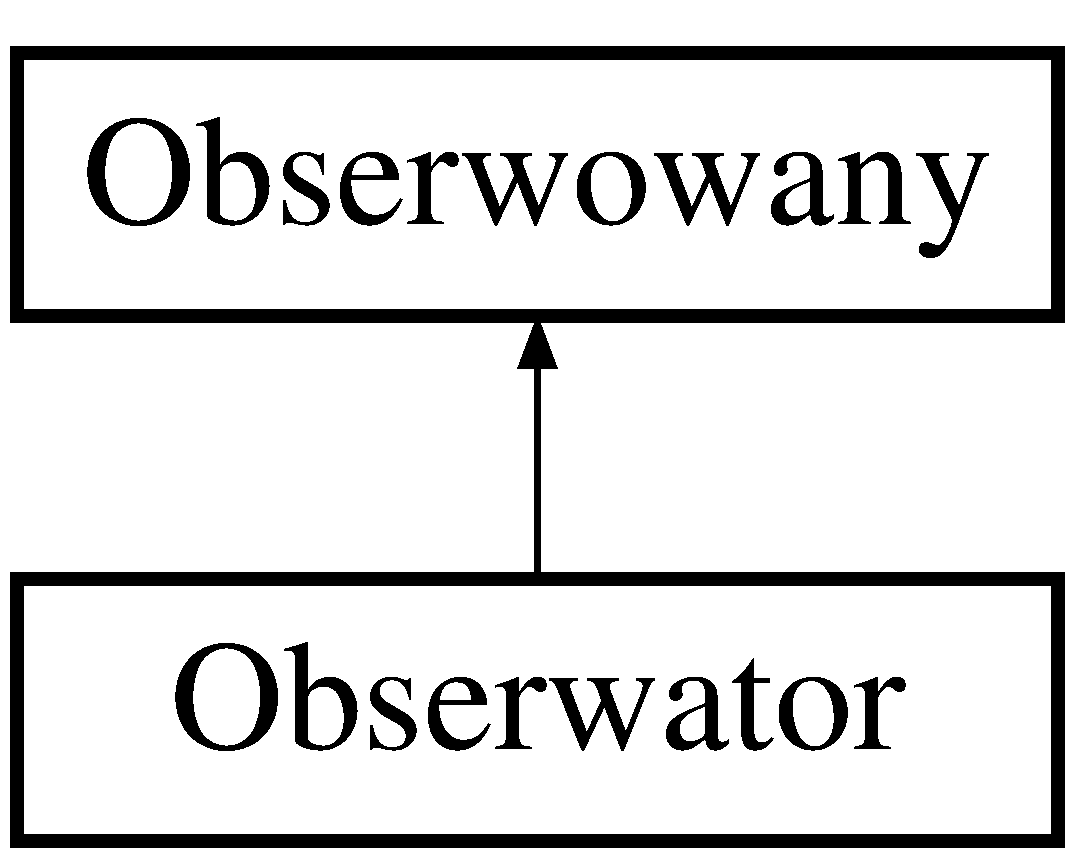
\includegraphics[height=2.000000cm]{class_obserwowany}
\end{center}
\end{figure}
\subsection*{Public Member Functions}
\begin{DoxyCompactItemize}
\item 
virtual \hyperlink{class_obserwowany_a7868c0f4787b967b342593ad0f892097}{$\sim$\-Obserwowany} ()
\begin{DoxyCompactList}\small\item\em Wirtualny destruktor klasy \hyperlink{class_obserwowany}{Obserwowany}. \end{DoxyCompactList}\item 
virtual void \hyperlink{class_obserwowany_a69ec45dd98ed98aeb1fcaf403bf04883}{dodaj} (\hyperlink{class_dane}{Dane} $\ast$o)
\begin{DoxyCompactList}\small\item\em Wirtualna funkcja dodajaca obserwatora. \end{DoxyCompactList}\item 
virtual void \hyperlink{class_obserwowany_a1ff3e88798e13410084c0795d99eded3}{usun} (\hyperlink{class_dane}{Dane} $\ast$o)
\begin{DoxyCompactList}\small\item\em Wirtualna funkcja usuwajaca obserwatora. \end{DoxyCompactList}\item 
virtual void \hyperlink{class_obserwowany_a8ffc862a3ea11828b24597888f3c7f7b}{przekaz} ()
\begin{DoxyCompactList}\small\item\em Wirtualna funkcja przekazujaca dane do wszystkicj obserwatorow. \end{DoxyCompactList}\end{DoxyCompactItemize}


\subsection{Detailed Description}
Definicja klasy \hyperlink{class_obserwowany}{Obserwowany}. 

Prywatnie zawiera liste wskaznikow na obserwatorow typu \hyperlink{class_dane}{Dane} 

Definition at line 46 of file Benchmark.\-h.



\subsection{Constructor \& Destructor Documentation}
\hypertarget{class_obserwowany_a7868c0f4787b967b342593ad0f892097}{\index{Obserwowany@{Obserwowany}!$\sim$\-Obserwowany@{$\sim$\-Obserwowany}}
\index{$\sim$\-Obserwowany@{$\sim$\-Obserwowany}!Obserwowany@{Obserwowany}}
\subsubsection[{$\sim$\-Obserwowany}]{\setlength{\rightskip}{0pt plus 5cm}virtual Obserwowany\-::$\sim$\-Obserwowany (
\begin{DoxyParamCaption}
{}
\end{DoxyParamCaption}
)\hspace{0.3cm}{\ttfamily [inline]}, {\ttfamily [virtual]}}}\label{class_obserwowany_a7868c0f4787b967b342593ad0f892097}


Wirtualny destruktor klasy \hyperlink{class_obserwowany}{Obserwowany}. 



Definition at line 58 of file Benchmark.\-h.



\subsection{Member Function Documentation}
\hypertarget{class_obserwowany_a69ec45dd98ed98aeb1fcaf403bf04883}{\index{Obserwowany@{Obserwowany}!dodaj@{dodaj}}
\index{dodaj@{dodaj}!Obserwowany@{Obserwowany}}
\subsubsection[{dodaj}]{\setlength{\rightskip}{0pt plus 5cm}virtual void Obserwowany\-::dodaj (
\begin{DoxyParamCaption}
\item[{{\bf Dane} $\ast$}]{o}
\end{DoxyParamCaption}
)\hspace{0.3cm}{\ttfamily [inline]}, {\ttfamily [virtual]}}}\label{class_obserwowany_a69ec45dd98ed98aeb1fcaf403bf04883}


Wirtualna funkcja dodajaca obserwatora. 


\begin{DoxyParams}[1]{Parameters}
\mbox{\tt in}  & {\em o} & -\/ dodawany obserwator typu Dane$\ast$ \\
\hline
\end{DoxyParams}


Definition at line 66 of file Benchmark.\-h.

\hypertarget{class_obserwowany_a8ffc862a3ea11828b24597888f3c7f7b}{\index{Obserwowany@{Obserwowany}!przekaz@{przekaz}}
\index{przekaz@{przekaz}!Obserwowany@{Obserwowany}}
\subsubsection[{przekaz}]{\setlength{\rightskip}{0pt plus 5cm}virtual void Obserwowany\-::przekaz (
\begin{DoxyParamCaption}
{}
\end{DoxyParamCaption}
)\hspace{0.3cm}{\ttfamily [inline]}, {\ttfamily [virtual]}}}\label{class_obserwowany_a8ffc862a3ea11828b24597888f3c7f7b}


Wirtualna funkcja przekazujaca dane do wszystkicj obserwatorow. 



Definition at line 87 of file Benchmark.\-h.

\hypertarget{class_obserwowany_a1ff3e88798e13410084c0795d99eded3}{\index{Obserwowany@{Obserwowany}!usun@{usun}}
\index{usun@{usun}!Obserwowany@{Obserwowany}}
\subsubsection[{usun}]{\setlength{\rightskip}{0pt plus 5cm}virtual void Obserwowany\-::usun (
\begin{DoxyParamCaption}
\item[{{\bf Dane} $\ast$}]{o}
\end{DoxyParamCaption}
)\hspace{0.3cm}{\ttfamily [inline]}, {\ttfamily [virtual]}}}\label{class_obserwowany_a1ff3e88798e13410084c0795d99eded3}


Wirtualna funkcja usuwajaca obserwatora. 


\begin{DoxyParams}[1]{Parameters}
\mbox{\tt in}  & {\em o} & -\/ usuwany obserwator typu Dane$\ast$ \\
\hline
\end{DoxyParams}


Definition at line 77 of file Benchmark.\-h.



The documentation for this class was generated from the following file\-:\begin{DoxyCompactItemize}
\item 
/home/damian/prog/\-Obserwator/prj/inc/\hyperlink{_benchmark_8h}{Benchmark.\-h}\end{DoxyCompactItemize}

\hypertarget{class_pobieracz_danych}{\section{Pobieracz\-Danych Class Reference}
\label{class_pobieracz_danych}\index{Pobieracz\-Danych@{Pobieracz\-Danych}}
}


Definicja klasy \hyperlink{class_pobieracz_danych}{Pobieracz\-Danych}.  




{\ttfamily \#include $<$Benchmark.\-h$>$}

Inheritance diagram for Pobieracz\-Danych\-:\begin{figure}[H]
\begin{center}
\leavevmode
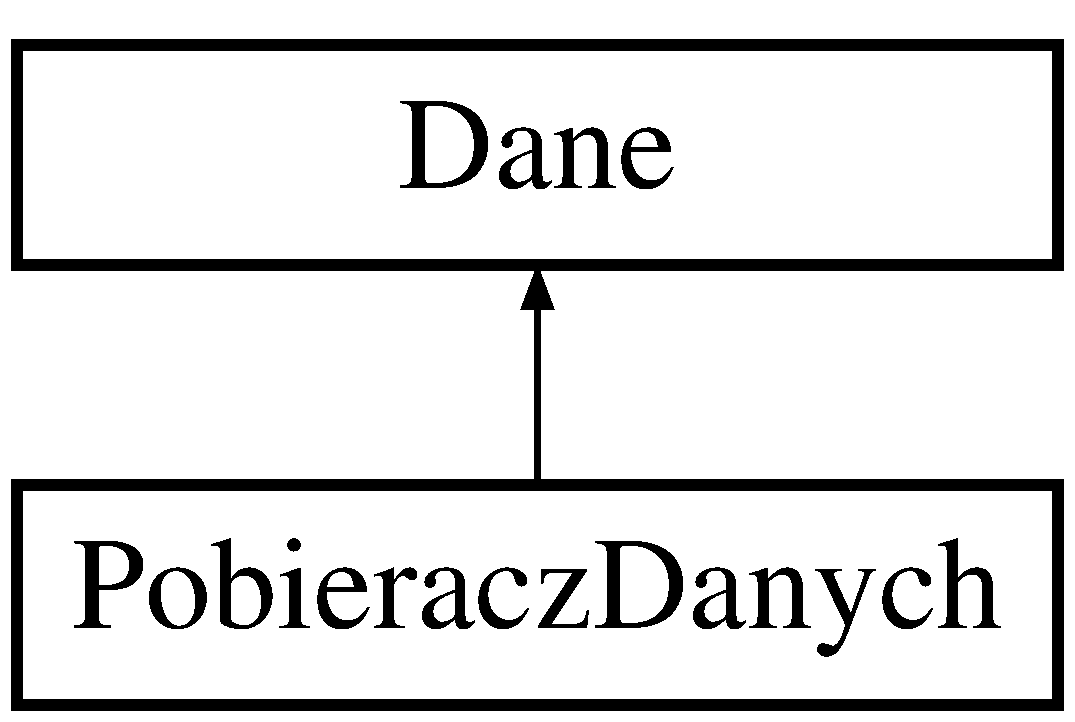
\includegraphics[height=2.000000cm]{class_pobieracz_danych}
\end{center}
\end{figure}
\subsection*{Public Member Functions}
\begin{DoxyCompactItemize}
\item 
virtual void \hyperlink{class_pobieracz_danych_a36a1901f8c7f9228f90c713a8e267b98}{update} (\hyperlink{class_obserwowany}{Obserwowany} $\ast$O)
\end{DoxyCompactItemize}


\subsection{Detailed Description}
Definicja klasy \hyperlink{class_pobieracz_danych}{Pobieracz\-Danych}. 

Zawiera jedna metode wirtualna ktora uaktualnia dane w Obserwatorach oraz wypisuje noew dane. Kazdy obserwator wypisuje raz swoje dane. 

Definition at line 176 of file Benchmark.\-h.



\subsection{Member Function Documentation}
\hypertarget{class_pobieracz_danych_a36a1901f8c7f9228f90c713a8e267b98}{\index{Pobieracz\-Danych@{Pobieracz\-Danych}!update@{update}}
\index{update@{update}!PobieraczDanych@{Pobieracz\-Danych}}
\subsubsection[{update}]{\setlength{\rightskip}{0pt plus 5cm}virtual void Pobieracz\-Danych\-::update (
\begin{DoxyParamCaption}
\item[{{\bf Obserwowany} $\ast$}]{O}
\end{DoxyParamCaption}
)\hspace{0.3cm}{\ttfamily [inline]}, {\ttfamily [virtual]}}}\label{class_pobieracz_danych_a36a1901f8c7f9228f90c713a8e267b98}


Implements \hyperlink{class_dane_a45055e5aa4e72fbb3a0717447fafbe75}{Dane}.



Definition at line 178 of file Benchmark.\-h.



The documentation for this class was generated from the following file\-:\begin{DoxyCompactItemize}
\item 
/home/damian/prog/\-Obserwator/prj/inc/\hyperlink{_benchmark_8h}{Benchmark.\-h}\end{DoxyCompactItemize}

\chapter{File Documentation}
\section{/home/damian/prog/graf/prj/inc/\-Benchmark.h File Reference}
\label{_benchmark_8h}\index{/home/damian/prog/graf/prj/inc/\-Benchmark.\-h@{/home/damian/prog/graf/prj/inc/\-Benchmark.\-h}}


Plik naglowkowy \doxyref{Benchmark.\-h}{p.}{_benchmark_8h}.  


{\ttfamily \#include \char`\"{}operacja.\-h\char`\"{}}\\*
{\ttfamily \#include \char`\"{}graff.\-h\char`\"{}}\\*
{\ttfamily \#include $<$list$>$}\\*
{\ttfamily \#include $<$ctime$>$}\\*
{\ttfamily \#include $<$cstdlib$>$}\\*
{\ttfamily \#include $<$unistd.\-h$>$}\\*
\subsection*{Classes}
\begin{DoxyCompactItemize}
\item 
class {\bf Dane}
\begin{DoxyCompactList}\small\item\em Deklaracja klasy \doxyref{Dane}{p.}{class_dane}. \end{DoxyCompactList}\item 
class {\bf Obserwowany}
\begin{DoxyCompactList}\small\item\em Definicja klasy \doxyref{Obserwowany}{p.}{class_obserwowany}. \end{DoxyCompactList}\item 
class {\bf Obserwator}
\begin{DoxyCompactList}\small\item\em Definicja klasy \doxyref{Obserwator}{p.}{class_obserwator}. \end{DoxyCompactList}\item 
class {\bf Pobieracz\-Danych}
\begin{DoxyCompactList}\small\item\em Definicja klasy \doxyref{Pobieracz\-Danych}{p.}{class_pobieracz_danych}. \end{DoxyCompactList}\end{DoxyCompactItemize}


\subsection{Detailed Description}
Plik naglowkowy \doxyref{Benchmark.\-h}{p.}{_benchmark_8h}. Zawiera klasy \doxyref{Obserwowany}{p.}{class_obserwowany},\doxyref{Obserwator}{p.}{class_obserwator},\doxyref{Dane}{p.}{class_dane} oraz \doxyref{Pobieracz\-Danych}{p.}{class_pobieracz_danych} i ich metody 

Definition in file {\bf Benchmark.\-h}.


\hypertarget{_lista_ar_8h}{\section{/home/damian/prog/praca na zajeciach(nowy sort)/prj/inc/\-Lista\-Ar.h File Reference}
\label{_lista_ar_8h}\index{/home/damian/prog/praca na zajeciach(nowy sort)/prj/inc/\-Lista\-Ar.\-h@{/home/damian/prog/praca na zajeciach(nowy sort)/prj/inc/\-Lista\-Ar.\-h}}
}


Plik naglowkowy \hyperlink{_lista_ar_8h}{Lista\-Ar.\-h}.  


{\ttfamily \#include $<$iostream$>$}\\*
\subsection*{Classes}
\begin{DoxyCompactItemize}
\item 
class \hyperlink{class_ltab}{Ltab}
\begin{DoxyCompactList}\small\item\em Modeluje pojecie klasy \hyperlink{class_ltab}{Ltab}. \end{DoxyCompactList}\end{DoxyCompactItemize}


\subsection{Detailed Description}
Plik naglowkowy \hyperlink{_lista_ar_8h}{Lista\-Ar.\-h}. Zawiera klase \hyperlink{class_ltab}{Ltab} i jej metody 

Definition in file \hyperlink{_lista_ar_8h_source}{Lista\-Ar.\-h}.


\hypertarget{operacja_8h}{\section{/home/damian/prog/\-Obserwator/prj/inc/operacja.h File Reference}
\label{operacja_8h}\index{/home/damian/prog/\-Obserwator/prj/inc/operacja.\-h@{/home/damian/prog/\-Obserwator/prj/inc/operacja.\-h}}
}
{\ttfamily \#include \char`\"{}Lista\-Ar.\-h\char`\"{}}\\*
\subsection*{Functions}
\begin{DoxyCompactItemize}
\item 
\hyperlink{class_ltab}{Ltab} \hyperlink{operacja_8h_a55fd4ff5b64240f5b5e352bf951d0eaf}{operacja} (\hyperlink{class_ltab}{Ltab} A, int l, int p)
\end{DoxyCompactItemize}


\subsection{Function Documentation}
\hypertarget{operacja_8h_a55fd4ff5b64240f5b5e352bf951d0eaf}{\index{operacja.\-h@{operacja.\-h}!operacja@{operacja}}
\index{operacja@{operacja}!operacja.h@{operacja.\-h}}
\subsubsection[{operacja}]{\setlength{\rightskip}{0pt plus 5cm}{\bf Ltab} operacja (
\begin{DoxyParamCaption}
\item[{{\bf Ltab}}]{A, }
\item[{int}]{l, }
\item[{int}]{p}
\end{DoxyParamCaption}
)}}\label{operacja_8h_a55fd4ff5b64240f5b5e352bf951d0eaf}


Definition at line 10 of file operacja.\-cpp.


\hypertarget{_benchmark_8cpp}{\section{/home/damian/prog/\-Obserwator/prj/src/\-Benchmark.cpp File Reference}
\label{_benchmark_8cpp}\index{/home/damian/prog/\-Obserwator/prj/src/\-Benchmark.\-cpp@{/home/damian/prog/\-Obserwator/prj/src/\-Benchmark.\-cpp}}
}


Plik \hyperlink{_benchmark_8cpp}{Benchmark.\-cpp}.  


{\ttfamily \#include \char`\"{}Benchmark.\-h\char`\"{}}\\*


\subsection{Detailed Description}
Plik \hyperlink{_benchmark_8cpp}{Benchmark.\-cpp}. Zawiera definicje metod klas \hyperlink{class_obserwator}{Obserwator}, \hyperlink{class_obserwowany}{Obserwowany}. 

Definition in file \hyperlink{_benchmark_8cpp_source}{Benchmark.\-cpp}.


\hypertarget{_lista_ar_8cpp}{\section{/home/damian/prog/praca na zajeciach(nowy sort)/\-Sortowania(wybrany-\/przez wstawianie)/prj/src/\-Lista\-Ar.cpp File Reference}
\label{_lista_ar_8cpp}\index{/home/damian/prog/praca na zajeciach(nowy sort)/\-Sortowania(wybrany-\/przez wstawianie)/prj/src/\-Lista\-Ar.\-cpp@{/home/damian/prog/praca na zajeciach(nowy sort)/\-Sortowania(wybrany-\/przez wstawianie)/prj/src/\-Lista\-Ar.\-cpp}}
}


Plik \hyperlink{_lista_ar_8cpp}{Lista\-Ar.\-cpp}.  


{\ttfamily \#include \char`\"{}Lista\-Ar.\-h\char`\"{}}\\*
{\ttfamily \#include $<$cstdlib$>$}\\*


\subsection{Detailed Description}
Plik \hyperlink{_lista_ar_8cpp}{Lista\-Ar.\-cpp}. Zawiera definicje metod klasy \hyperlink{class_ltab}{Ltab} 

Definition in file \hyperlink{_lista_ar_8cpp_source}{Lista\-Ar.\-cpp}.


\hypertarget{main_8cpp}{\section{/home/damian/prog/praca na zajeciach(nowy sort)/prj/src/main.cpp File Reference}
\label{main_8cpp}\index{/home/damian/prog/praca na zajeciach(nowy sort)/prj/src/main.\-cpp@{/home/damian/prog/praca na zajeciach(nowy sort)/prj/src/main.\-cpp}}
}
{\ttfamily \#include \char`\"{}Lista\-Ar.\-h\char`\"{}}\\*
{\ttfamily \#include $<$ctime$>$}\\*
\subsection*{Functions}
\begin{DoxyCompactItemize}
\item 
int \hyperlink{main_8cpp_ae66f6b31b5ad750f1fe042a706a4e3d4}{main} ()
\end{DoxyCompactItemize}


\subsection{Function Documentation}
\hypertarget{main_8cpp_ae66f6b31b5ad750f1fe042a706a4e3d4}{\index{main.\-cpp@{main.\-cpp}!main@{main}}
\index{main@{main}!main.cpp@{main.\-cpp}}
\subsubsection[{main}]{\setlength{\rightskip}{0pt plus 5cm}int main (
\begin{DoxyParamCaption}
{}
\end{DoxyParamCaption}
)}}\label{main_8cpp_ae66f6b31b5ad750f1fe042a706a4e3d4}


Definition at line 7 of file main.\-cpp.


\section{/home/damian/prog/graf/prj/src/operacja.cpp File Reference}
\label{operacja_8cpp}\index{/home/damian/prog/graf/prj/src/operacja.\-cpp@{/home/damian/prog/graf/prj/src/operacja.\-cpp}}


Plik \doxyref{operacja.\-cpp}{p.}{operacja_8cpp}.  


{\ttfamily \#include \char`\"{}operacja.\-h\char`\"{}}\\*
\subsection*{Functions}
\begin{DoxyCompactItemize}
\item 
void {\bf operacja} ({\bf Graf} A, int poczatek, int opcja)
\begin{DoxyCompactList}\small\item\em Funkcja operacja. \end{DoxyCompactList}\end{DoxyCompactItemize}


\subsection{Detailed Description}
Plik \doxyref{operacja.\-cpp}{p.}{operacja_8cpp}. Zawiera definicje funkcji operacja wykonywanej na liscie. 

Definition in file {\bf operacja.\-cpp}.



\subsection{Function Documentation}
\index{operacja.\-cpp@{operacja.\-cpp}!operacja@{operacja}}
\index{operacja@{operacja}!operacja.cpp@{operacja.\-cpp}}
\subsubsection[{operacja}]{\setlength{\rightskip}{0pt plus 5cm}void operacja (
\begin{DoxyParamCaption}
\item[{{\bf Graf}}]{A, }
\item[{int}]{poczatek, }
\item[{int}]{opcja}
\end{DoxyParamCaption}
)}\label{operacja_8cpp_a36acec75c8ad7a4cc3f25f08e27af5c7}


Funkcja operacja. 

Wykonuje zadana operacje na grafie


\begin{DoxyParams}[1]{Parameters}
\mbox{\tt in}  & {\em A} & -\/ Zadany graf o dowolnej ilosci wierzcholkow i krawedzi \\
\hline
\mbox{\tt in}  & {\em poczatek} & -\/ wierzcholek z ktorego zaczynamy przechodzenie Grafu \\
\hline
\mbox{\tt in}  & {\em opcja} & -\/ =1 gdy D\-F\-S =2 gdy B\-S\-F \\
\hline
\end{DoxyParams}


Definition at line 11 of file operacja.\-cpp.


%--- End generated contents ---

% Index
\newpage
\phantomsection
\addcontentsline{toc}{chapter}{Index}
\printindex

\end{document}
